%%==================================================
%% chapter03.tex for BIT Master Thesis
%% modified by yang yating
%% version: 0.1
%% last update: Dec 25th, 2016

%% modified by Meng Chao
%% version: 0.2
%% last update: May 29th, 2017
%%==================================================
\chapter{算法介绍}
\label{chap:ALGORITHM}
This chapter summaries the complete algorithm firstly, and introduce the information of the global mapping in the section A. In section B to section E, the tracking of new frames, depth information estimation, key frame matching and Map representation and optimization will be described.


%3.1
\section{The Algorithm Overview}
The LSD-SLAM contains three essential parts, which is tracking, depth information estimation and map optimization. The algorithm construct is displayed in Fig.2.

The tracking continuously tracks new camera images. It estimates their rigid body pose $\xi  \in se(3)$ about the current key frame, using the pose of the previous frame as initialization.

The depth information estimation uses tracked frames to either refine or replace the current key frame. Depth is refined by filtering over many per-pixel, small-baseline stereo comparisons coupled with interleaved spatial regularization [5]. Once a key frame is replaced as tracking reference and hence its depth information will not be refined further. It is combined the global map by the map optimization.

The map is represented as a pose graph of key frames. This paper will keep correspondence with the convenient for describe [1]. Each key frame ${k_i}$ consists of a image ${I_i}$, an inverse depth information ${D_i}$ and the variance of the inverse depth ${V_i}$. Note that the depth information and variance are only defined for a subset of pixels ${\Omega _{{D_i}}} \in {\Omega _i}$ containing all image regions in the vicinity of sufficiently large intensity gradient. Edges ${\varepsilon _{ji}}$ between key frames contain their relative alignment as similarity transform ${\xi _{ji}} \in sim(3)$, as well as the corresponding covariance matrix ${\Sigma _{ji}}$.

\begin{figure}
  \centering
  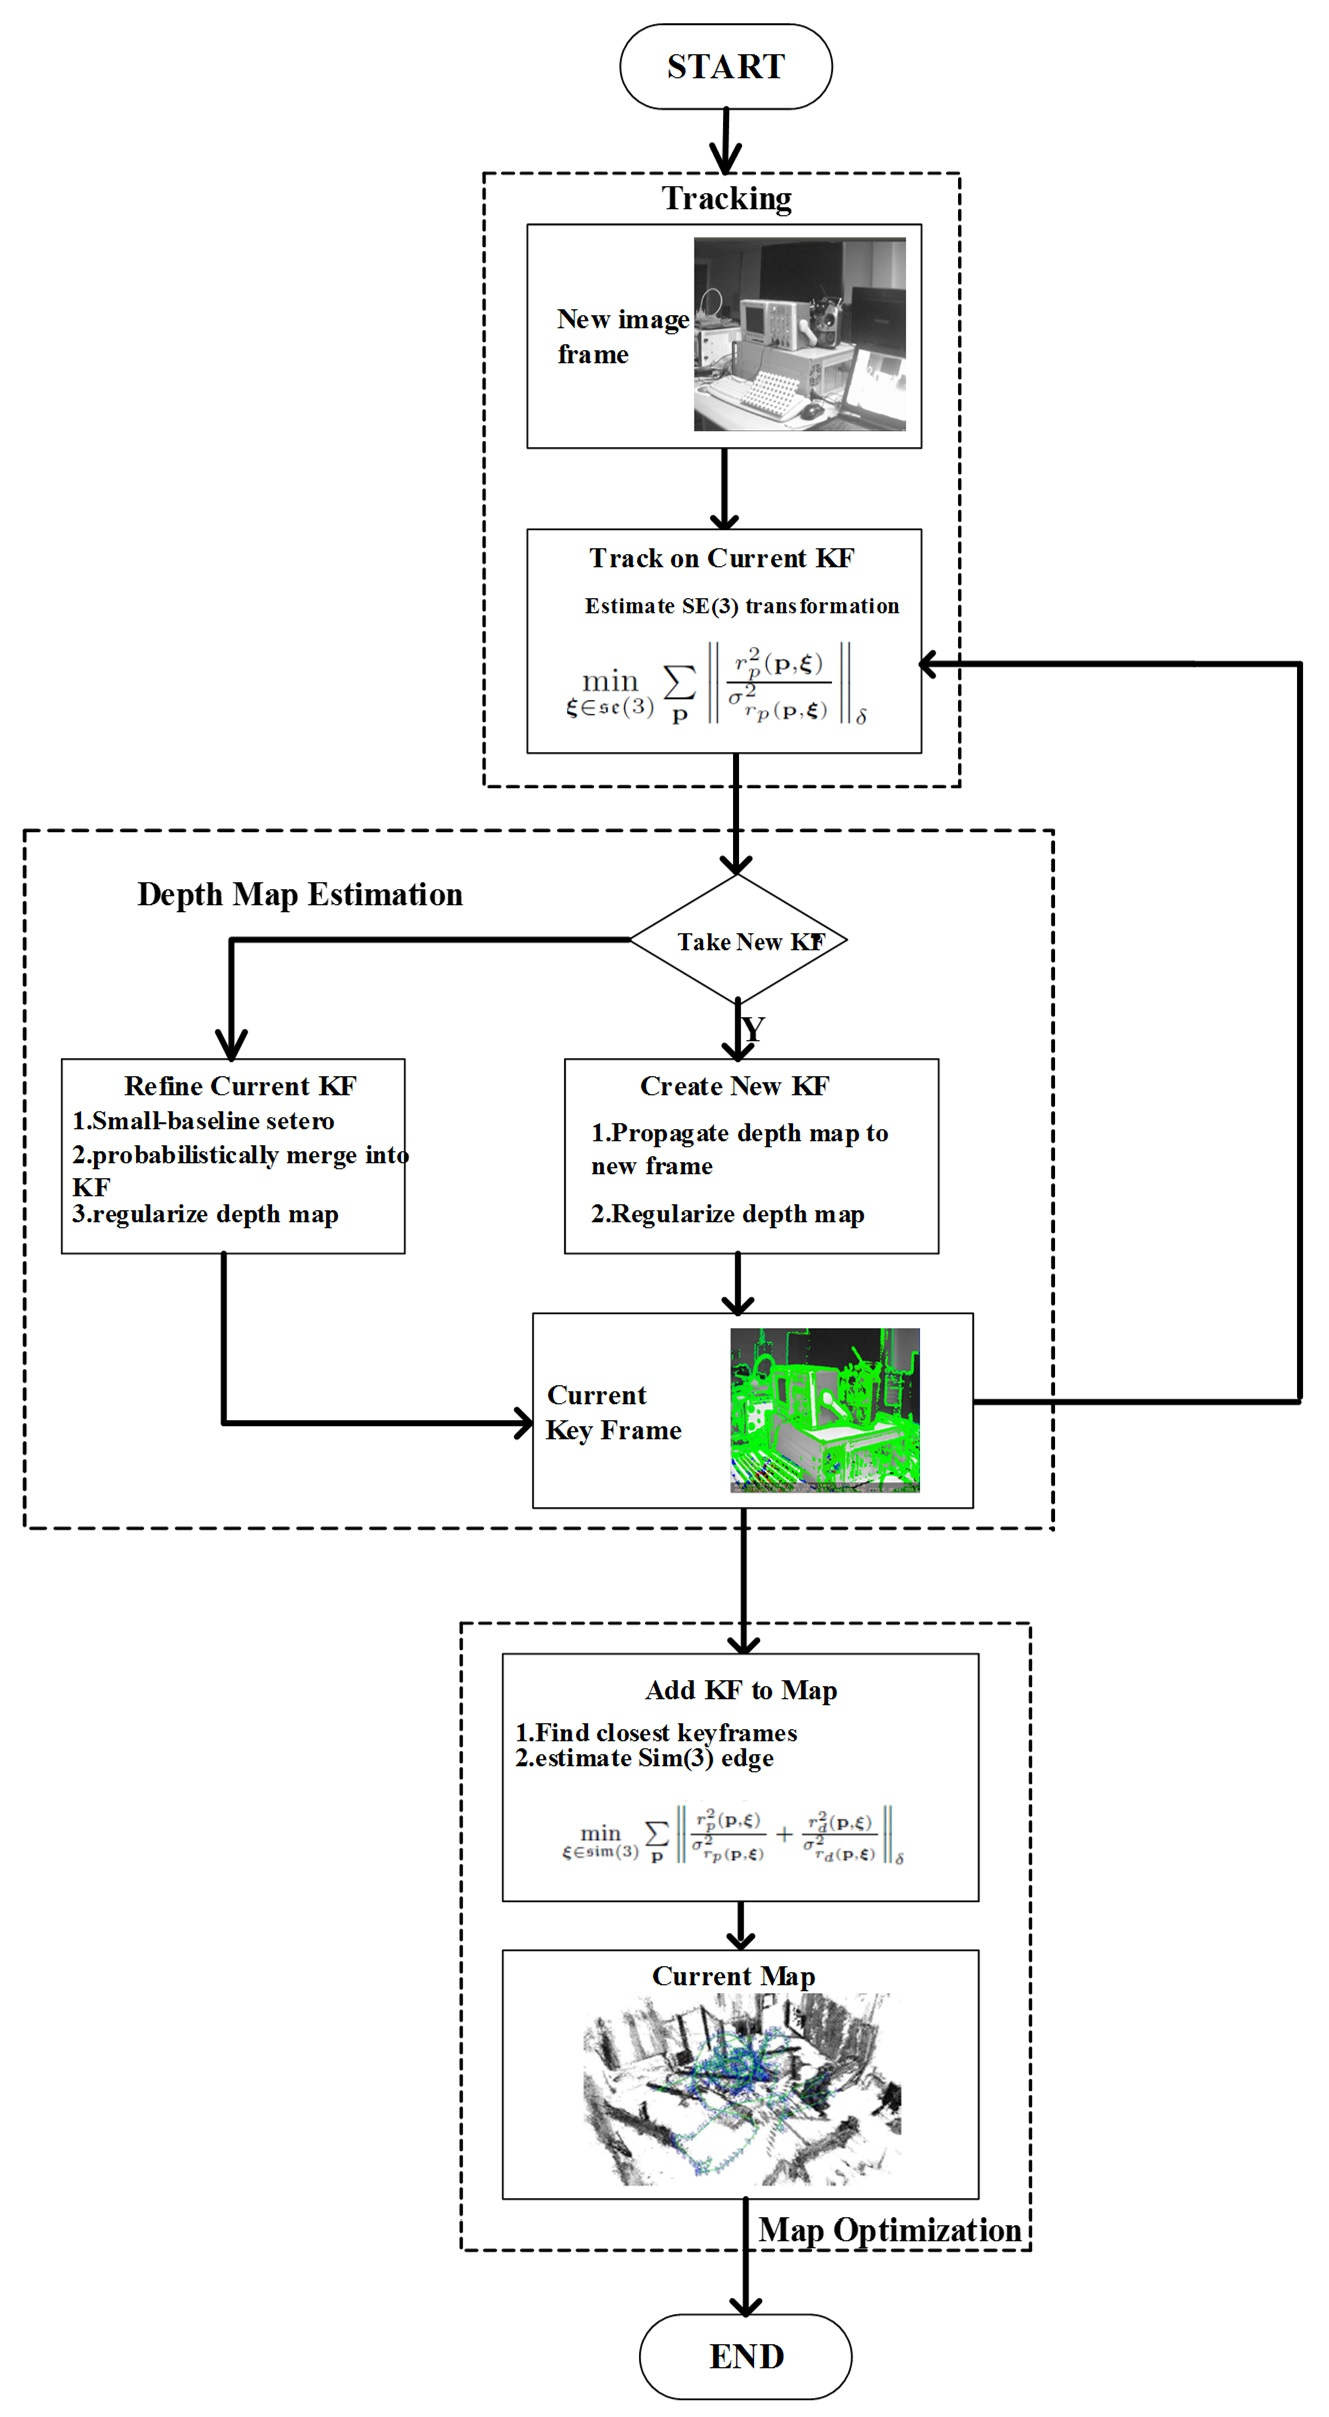
\includegraphics[width=0.4\textwidth, height=0.6\textwidth]{figures/Fig2}
  \caption{Overview of LSD-SLAM}
  %\label{referencename};
\end{figure}

The LSD-SLAM complete working flow and algorithm processing is displayed in Figure 3.

\begin{figure}
  \centering
  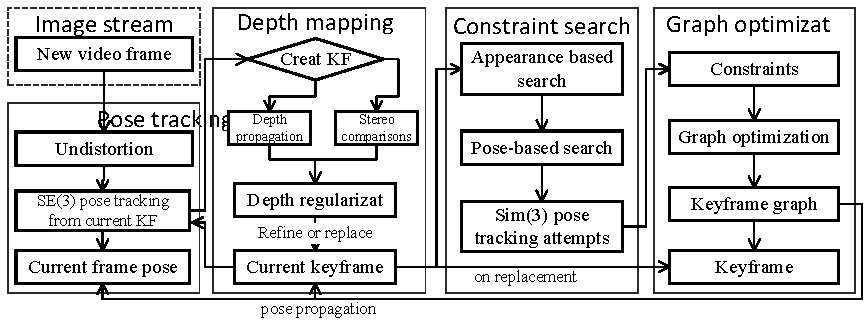
\includegraphics[width=0.45\textwidth]{figures/Fig3(2)}
  \caption{LSD-SLAM working flow}
  %\label{referencename};
\end{figure}


%3.2
\section{Tracking New Frames}
The current frames will replace the current key frames according with the Direct SE(3) image alignment. An existing key frame ${k_i} = ({I_i},{D_i},{V_i})$, the relative posture ${\xi _{ji}} \in se(3)$ of a new image ${I_j}$ is obtained by minimizing the variance-normalized photometric error

\begin{equation}
E_{p}(\xi _{ji}) = \sum\limits_{p \in \Omega _{D_{i}}} \left\|  \frac{r_{p}^{2} (p,\xi_{ji})}{\sigma_{r_{p}}^{2} (p,\xi_{ji})}  \right\|_{\delta}
\end{equation}


\begin{equation}
r_{p}(p,\xi _{ji}): = I_{i}(p) - I_{j}(\omega (p,D_{i}(p),\xi _{ji}))
\end{equation}

\begin{equation}
\sigma _{r_{p}} ^{2}(p,\xi _{ji}): = 2\sigma _{I} ^{2} + {\left( \frac {\partial r_{p}(p,\xi_{ji})} {\partial D_{i} (p)} \right)^{2}} V_{i}(p)
\end{equation}

The formula (13) is the Huber norm and applied to the normalized residual.

\begin{equation}
{\left\| r^{2} \right\|_{\delta}}:=\left\{\begin{array}{ll}
\frac {r^{2}} {2\delta}            & |r|\leq \delta       \\
|r|-\frac {\delta} {2}      & |r| > \delta
\end{array} \right.
\end{equation}


%3.3
\section{Depth Map Estimation}
If the camera moves too far away from the existing map, a new key frame is created from the most recent tracked image. We threshold a weighted combination of relative distance and angle to the current key frame

\begin{equation}
dist({\xi _{ji}}): = \xi _{ji}^TW{\xi _{ji}}
\end{equation}

Where W is a diagonal matrix containing the weights. Note that, as described in the following section, each key frame is scaled such that its mean inverse depth is one. This threshold is therefore relative to the current scale of the scene, and ensures sufficient possibilities for small-baseline stereo comparisons.

Once a new frame is chosen to become a key frame, its depth map is initialized by projecting points from the previous key frame into it, followed by one iteration of spatial regularization and outlier removal [5]. Afterwards, the depth map is scaled to have a mean inverse depth of one -this scaling factor is directly incorporated into the sim(3) camera pose. Finally, it replaces the previous key frame and is used for tracking subsequent new frames.


%3.4
\section{Direct Image Alignment}
In contrast to RGB-D or Stereo SLAM, monocular SLAM is inherently scale-ambivalent, the absolute scale of the world is not observable. Over long trajectories this leads to scale-drift, which is one of the major sources of error [9]. Further, all distances are only defined up to scale, which causes threshold-based outlier rejection or parametrized robust kernels to be ill-defined.

We select an advanced method in [1] for better perform direct, scale-drift image alignment, which is used to align two differently scaled key frames. For the photometric residual ${r_p}$, the depth residual ${r_d}$ which penalizes deviations in inverse depth between key frames, allowing to directly estimate the scaled transformation between them. The total error function becomes

\begin{equation}
E({\xi _{ji}}): = {\sum\limits_{p \in {\Omega _{{D_i}}}} {\left\| {\frac{{r_p^2(p,{\xi _{ji}})}}{{\sigma _{{r_p}(p,{\xi _{ji}})}^2}} + \frac{{r_d^2(p,{\xi _{ji}})}}{{\sigma _{{r_d}(p,{\xi _{ji}})}^2}}} \right\|} _\delta }
\end{equation}
the depth residual is computed

\begin{equation}
r_{d}(p,\xi _{ji}): = [p^{'}]_{3} - D_{j}([p^{'}]_{1,2})
\end{equation}

% 公式换行用 \\ 
\begin{equation}
\begin{split}
\sigma_{r_{d}(p,\xi_{ji})} ^{2} :=V_{j}( [ p^{'} ]_{1,2} )  {\left( \frac {\partial r_{d}(p,\xi_{ji})} {\partial D_{j} \left[ p^{'} \right]_{1,2}}  \right)^{2}} + V_{i}(p) \left( \frac {\partial r_{d}(p,\xi_{ji})} {\partial D_{j}(p)} \right)
\end{split}
\end{equation}

After a new key frame ${k_i}$ is added to the map, a number of possible loop closure key frames ${k_{ji}},....{k_{jn}}$ is collected. We use the closet ten key frames, as well as a suitable candidate. To avoid insertion of false or falsely tracked loop closures, we then perform a reciprocal tracking check. For each candidate ${k_{jk}}$ we independently track ${\xi _{{j_k}i}}$ and ${\xi _{i{j_k}}}$.

\begin{equation}
e\!(\!{\xi _{{j_k}i}},{\xi _{i{j_k}}})\!: \!= \!{\!(\!{\xi _{{j_k}i}} \!\circ \!{\xi _{i{j_k}}})\!^T}{\!(\!{\Sigma _{{j_k}i}}\! +\! Ad{j_{{j_k}i}}{\Sigma _{i{j_k}}}Adj_{{j_k}i}^T\!)\!^{ - 1}}\!(\!{\xi _{{j_k}i}}\! \circ\! {\xi _{i{j_k}}}\!)
\end{equation}

Only if the two estimates are statistically similar, if formula (18) is sufficiently small, they are added to the global map. For this, the adjoint $Ad{j_{{j_k}i}}$ is used to transform ${\Sigma _{i{j_k}}}$ into the correct tangent space.


%3.5
\section{Map Representation and Optimization}
The map is represented as a pose graph of keyframes: Each keyframe $\kappa_{i}$ consists of a camera image $I_{i}\!:\!\Omega_{D_{i}}\!\rightarrow \!{\mathbb{R}}$,an inverse depth map $D_{i}\!:\!\Omega_{D_{i}}\!\rightarrow \!{\mathbb{R}}^{+}$, and the variance of the inverse depth $ V_{i}\!:\!\Omega_{D_{i}}\!\rightarrow \!{\mathbb{R}}^{+}$.Note that the depth map and variance are only defined for a subset of pixels $ \Omega_{D_{i}}\!\subset\!\Omega_{i} $, containing all image regions in the vicinity of sufficiently large intensity gradient, hence semi-dense.Edges $ \varepsilon_{ji}$ between keyframes contain their relative alignment as similarity transform $ \xi_{ji}\in sim(3) $, as well as the corresponding covariance matrix $\Sigma_{ji} $

The map, consisting of a set of keyframes and tracked sim(3)-constraints, is continuously optimized in the background using pose graph optimization. The
error function that is minimized is in accordance with the left-multiplication convention
\begin{equation}
E(\xi\!_{W\!_{1}}\!...\!\xi\!_{W\!_{n}})\!:\!= \sum\limits_{(\!\xi\!_{ji},\Sigma\!_{ji}\!)\!\in\!\varepsilon}\!(\!\xi_{ji}\!\circ\!\xi_{\!W_{i}\!}^{-1}\! \!\circ\!\xi_{\!W\!_{j}}\!)\!^{T}\!\Sigma_{\!j\!i}^{\!-1\!}\!(\!\xi_{ji}\!\circ\!\xi_{\!W_{i}\!}^{-1}\! \!\circ\!\xi_{\!W\!_{j}}\!)
\end{equation}


